\documentclass[12pt, openany]{book}
\usepackage[lmargin = 3cm, rmargin = 3cm, top=2cm]{geometry}
\usepackage{listings}
\usepackage[normalem]{ulem}
\usepackage{graphicx}
\usepackage{float}
%\usepackage{pdflscape}
%\usepackage{afterpage}
\usepackage{footnote}
\usepackage{newfile}
\usepackage{currfile}

%Includes color package and defines suctom colors
\usepackage{xcolor}

\definecolor{codegreen}{rgb}{0,0.6,0}
\definecolor{textgreen}{rgb}{0,0.6,0}
\definecolor{textpurple}{rgb}{0.36,0.19,0.41}
\definecolor{warwickorange}{rgb}{0.96, 0.48, 0.13}
\definecolor{textblue}{rgb}{0.14, 0.34, 0.52}
\definecolor{warwickgold}{rgb}{0.53, 0.42, 0.07}
\definecolor{warwickred}{rgb}{0.54, 0.06, 0.17}
\definecolor{warwickgreen}{rgb}{0.47, 0.47, 0.02}
\definecolor{warwickblue}{rgb}{0.0, 0.70, 0.87}


%Include definitions for programming languages


%Fortran and C specific parts are coloured
\newcommand{\fortonly}[1]{\textcolor{textblue}{#1}}
\newcommand{\conly}[1]{\textcolor{warwickred}{#1}}

%Presenter/typesetter notes. Defaults to swallowing, swap to other to leave unchanged
\newcommand{\presnote}[1]{}
%\newcommand{\presnote}[1]{#1}

\newcommand{\aside}[1]{\emph{#1}}

%Extra emphasis
\newcommand{\superemph}[1]{\textcolor{red}{\emph{#1}}}

%Shaded aside boxes
\usepackage[breakable]{tcolorbox}
\newenvironment{asidebox}[1]{
	\begin{tcolorbox}[width=0.95\textwidth,colback={grey}, breakable, title=#1]}
{\end{tcolorbox}   
}

\lstdefinelanguage{pseudo}
{
morekeywords={FUNCTION, MODULE, BEGIN, END, PRINT, FOR, DO, IF, ELSE, THEN, RETURN, ASSERT, AND, OR},
morekeywords=[2]{MAIN, INTEGER, ARRAY,REAL, FLAG, STRING},
morekeywords=[3]{OPENW, OPENR, CLOSE, WRITE},
sensitive=true,
morecomment=[l]{//}
}
%Dummy docs language to get nice formatting and colours easily
\lstdefinelanguage{docs}
{
morekeywords={int, char, const, double, class, flag},
morekeywords=[2]{Parameters, Returns},
sensitive=true,
morecomment=[l]{\#}
}
\lstdefinelanguage{make}
{
morekeywords={target},
morekeywords=[2]{prerequisites},
morekeywords=[3]{recipe},
sensitive=false,
morecomment=[l]{\#}
}
\lstdefinelanguage{debug}
{
morekeywords={break, print, run, continue, if, delete, clear, quit},
morekeywords=[2]{gdb},
sensitive=true,
morecomment=[l]{\#}
}


\lstdefinestyle{pseudostyle}{
    language=pseudo,
    tabsize=3,
    frame=shadowbox,
    rulesepcolor=\color{gray},
    commentstyle=\color{codegreen},
    keywordstyle=\color{textblue}\bf,
    keywordstyle=[2]\color{textpurple}\bf,
    keywordstyle=[3]\color{warwickred}\bf,
    stringstyle=\color{warwickred},
    numbers=left,
    numberstyle=\tiny,
    numbersep=5pt,
    breaklines=true,
    showstringspaces=false,
    basicstyle=\footnotesize
    %emph={str},emphstyle={\color{magenta}}
  } 
\lstdefinestyle{docstyle}{
    language=docs,
    tabsize=3,
    frame=shadowbox,
    rulesepcolor=\color{gray},
    commentstyle=\color{codegreen},
    keywordstyle=\color{textblue}\bf,
    keywordstyle=[2]\color{textpurple}\bf,
    keywordstyle=[3]\color{warwickred}\bf,
    stringstyle=\color{warwickred},
    numbers=left,
    numberstyle=\tiny,
    numbersep=5pt,
    breaklines=true,
    showstringspaces=false,
    basicstyle=\footnotesize
  } 
\lstdefinestyle{debugstyle}{
    language=debug,
    tabsize=3,
    frame=shadowbox,
    rulesepcolor=\color{gray},
    commentstyle=\color{codegreen},
    keywordstyle=\color{textblue}\bf,
    keywordstyle=[2]\color{textpurple}\bf,
    stringstyle=\color{warwickred},
    numbers=left,
    numberstyle=\tiny,
    numbersep=5pt,
    breaklines=true,
    showstringspaces=false,
    basicstyle=\footnotesize
    %emph={str},emphstyle={\color{magenta}}
  } 

\lstdefinestyle{makestyle}{
    language=make,
    tabsize=3,
    frame=shadowbox,
    rulesepcolor=\color{gray},
    commentstyle=\color{codegreen},
    keywordstyle=\color{textblue}\bf,
    keywordstyle=[2]\color{textpurple}\bf,
    keywordstyle=[3]\color{warwickred}\bf,
    stringstyle=\color{warwickred},
    numbers=left,
    numberstyle=\tiny,
    numbersep=5pt,
    breaklines=true,
    showstringspaces=false,
    basicstyle=\footnotesize
    %emph={str},emphstyle={\color{magenta}}
  } 

\lstdefinestyle{nostyle}{
    tabsize=3,
    frame=shadowbox,
    rulesepcolor=\color{gray},
    commentstyle=\color{codegreen},
    keywordstyle=\color{textblue}\bf,
    keywordstyle=[2]\color{textpurple}\bf,
    stringstyle=\color{warwickred},
    numbers=left,
    numberstyle=\tiny,
    numbersep=5pt,
    breaklines=true,
    showstringspaces=false,
    basicstyle=\footnotesize
  } 

\lstdefinestyle{pystyle}{
    language=python,
    tabsize=3,
    frame=shadowbox,
    rulesepcolor=\color{gray},
    commentstyle=\color{codegreen},
    keywordstyle=\color{textblue}\bf,
    stringstyle=\color{warwickred},
    numbers=left,
    numberstyle=\tiny,
    numbersep=5pt,
    breaklines=true,
    showstringspaces=false,
    basicstyle=\footnotesize
  } 
\lstdefinestyle{forstyle}{
    language=fortran,
    tabsize=3,
    frame=shadowbox,
    rulesepcolor=\color{gray},
    commentstyle=\color{codegreen},
    keywordstyle=\color{textblue}\bf,
    stringstyle=\color{warwickred},
    numbers=left,
    numberstyle=\tiny,
    numbersep=5pt,
    breaklines=true,
    showstringspaces=false,
    basicstyle=\footnotesize
  } 
\lstdefinestyle{cstyle}{
    language=c,
    tabsize=3,
    frame=shadowbox,
    rulesepcolor=\color{gray},
    commentstyle=\color{codegreen},
    keywordstyle=\color{textblue}\bf,
    stringstyle=\color{warwickred}\bf,
    numbers=left,
    numberstyle=\tiny,
    numbersep=5pt,
    breaklines=true,
    showstringspaces=false,
    basicstyle=\footnotesize
  } 


%Fix splitting of URLs
\PassOptionsToPackage{hyphens}{url}\usepackage[colorlinks, linkcolor=warwickblue]{hyperref}

\usepackage[toc,section=section, seeautonumberlist]{glossaries}

\title{Title}
\author{CS Brady, H Ratcliffe}

%Fixes footnotes in tables
\makesavenoteenv{table}


\makenoidxglossaries
\loadglsentries{glossary_defs}

\begin{document}
%\maketitle
\begin{titlepage}
	\centering
	
\includegraphics[width=0.95\textwidth]{Warwick_A4_Bar}\par\vspace{1cm}
	{\scshape\LARGE Warwick Research Software Engineering \par}
	\vspace{1cm}
	{\huge\bfseries \newtitle \par}
	{\large\bfseries \newsubtitle \par}
	\vspace{2cm}
	{\Large\itshape \newauthor \par}
	Senior Research Software Engineers\par
	\vspace{3cm}
	
\includegraphics[width=0.25\textwidth]{WarwickRSE}\par\vspace{1cm}
	{\scriptsize ``The Angry Penguin'', used under creative commons licence\\
from Swantje Hess and Jannis Pohlmann.}

	\vfill

% Bottom of the page
	{\large \today\par}
\end{titlepage}

% Use \fbr{} to compile a list of things that should be fixed before these notes are released
% See these in  Main.FixBeforeRelease

\newoutputstream{thingsyoumustdo}
\immediate\openoutputfile{\jobname.must}{thingsyoumustdo}

%Must-do text effects
\newcommand{\musttext}[1]{\textcolor{red}{\textbf{#1}}}

%Must  text and file io
\newcommand{\mustnt}[1]{\musttext{#1}\addtostream{thingsyoumustdo}{\noexpand\item #1}}
\newcommand{\must}[1]{\mustnt{#1}}



\let\cleardoublepage\clearpage
\setcounter{tocdepth}{1}

\pagenumbering{gobble}
\tableofcontents

\frontmatter \chapter{Preface}
\section{About these Notes}
%My default preface
These notes were written by H Ratcliffe and C S Brady, both Senior Research Software Engineers in the Scientific Computing Research Technology Platform at the University of Warwick for a \fbr{Workshop first run in March 2020 at the University of Warwick}. 

%My default license
\textbf{This work, except where otherwise noted, is licensed under the Creative Commons Attribution-NonCommercial-NoDerivatives 4.0 International License. To view a copy of this license, visit \url{http://creativecommons.org/licenses/by-nc-nd/4.0/}}. 
\begin{figure}[h]
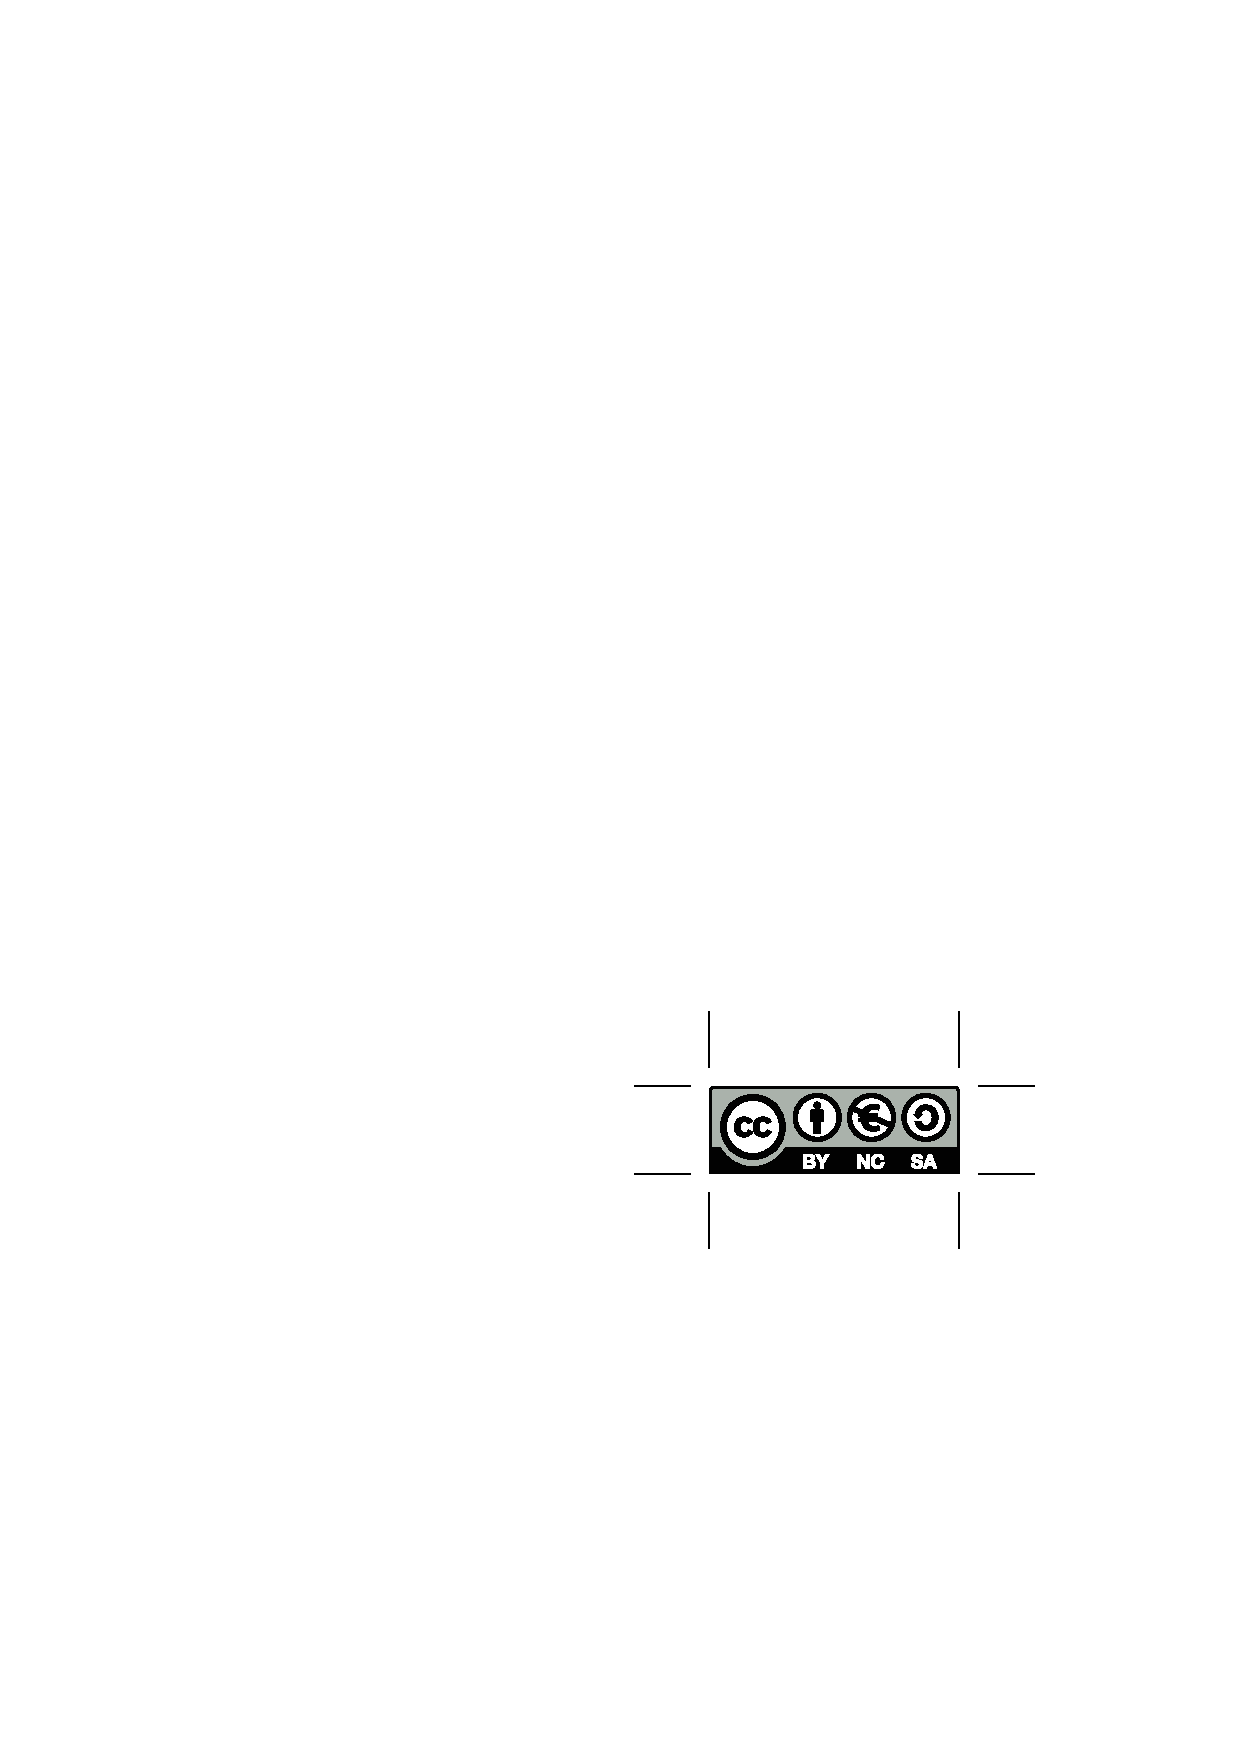
\includegraphics[width=0.15\textwidth]{by-nc-sa-eu}
\end{figure}

\noindent The notes may redistributed freely with attribution, but may not be used for commercial purposes nor altered or modified. The Angry Penguin and other reproduced material, is clearly marked in the text and is not included in this declaration. 

The notes  were typeset in \LaTeX by H Ratcliffe. \\Errors can be reported to \href{mailto:rse@warwick.ac.uk}{rse@warwick.ac.uk}

\subsection{Change Log}
\currfilename
Version 1 - date

\section{Example Programs}\label{sec:egCode}
Several sections of these notes benefit from a hands-on look at the concepts and tools involved. Test code is available on Github at \url{https://github.com/WarwickRSE/??}

\let\cleardoublepage\clearpage
\mainmatter

\chapter{Chapter Title}\label{chap:reference}
\section{Example}

Text here \gls{reference} \glspl{reference2}

\must{Something really important!} \should{something quite important}

\fbr{Insert figure here}

\begin{lstlisting}
CODE
\end{lstlisting}



\chapter{Summary}
\subsection{Wrap Up}

Example link: \href{https://warwick.ac.uk/research/rtp/sc/rse/training/hpcbeyond}{HPC at Warwick and Beyond}. 

%Close the streams for Must and Should so we can read from them below
\immediate\closeoutputstream{commandments}
\immediate\closeoutputstream{suggestions}

\chapter{Glossary of Terms}
%Include the glossary. Optionally can create multiple glossaries and insert only one type w. \printnoidxglossary[type=General]
\printnoidxglossary

%Optional - appendices
\appendix

%Include bullet lists of everything in must and should environments. Default titles Must and Should - change these or explain them in Intro
\chapter{Must and Shoulds}\label{sec:commandments}
\section{Must}
\begin{itemize}
    \input{\jobname.comm}
\end{itemize}

\section{Should}
\begin{itemize}
    \input{\jobname.sugg}
\end{itemize}

%Add all the glossary only terms (defined in glossary_defs but not used in text)
%Do this after all text etc, to get it right
\glsaddallunused


\end{document}